
\subsection{Method of Characteristics}

\textbf{Important:} Characteristics \textbf{cannot} be used as initial conditions, otherwise the characteristic becomes the solution (instead of obtaining a surface, you get a curve).\\
\textbf{Important:} The characteristic must pass through the boundary only once.\\
Useful for Quasilinear PDEs of 1st order. If separation is possible, this (simpler) method should be used.

Initial condition:
\[
    a(x,y,u)\cdot\partFrac{u}{x}+b(x,y,u)\cdot\partFrac{u}{y}-c(x,y,u)=0
\]
Characteristic:
\[
    \frac{d}{dt} \begin{bmatrix} x(t) \\ y(t) \\ u(t) \end{bmatrix}
    = \begin{bmatrix} a(x,y,u) \\ b(x,y,u) \\ c(x,y,u) \end{bmatrix}
\]


\begin{tabular}{ll}
Region:& $\Omega\{\ldots|x>0, \text{all }y\}$\qquad Boundary condition: $u(0,y_0)=g(y_0)$\\
Vector notation:& $\begin{bmatrix}
    a(x,y,u)\\ b(x,y,u)\\ c(x,y,u)
    \end{bmatrix}
\underset{\overrightarrow{n}\text{: Normal to surface}}{\underbrace{\begin{bmatrix}
\partFrac{u}{x} & \partFrac{u}{y} & -1
\end{bmatrix}}}=0 $ \\[1cm]
Tangents:& $\overrightarrow{t}_x=\begin{bmatrix}1\\0\\ \partFrac{u}{x}\end{bmatrix}\qquad
			\overrightarrow{t}_y=\begin{bmatrix}0\\1\\ \partFrac{u}{y}\end{bmatrix}\qquad \overrightarrow{n} \bullet \overrightarrow{t_x} = 0 \qquad \overrightarrow{n} \bullet \overrightarrow{t_y} = 0 \qquad \overrightarrow{t_x} \bullet \overrightarrow{t_y} = \overrightarrow{n}$\\[1cm]

Solution approach: & For each initial point $\begin{bmatrix} 0\\y_0\\g(y_0)\end{bmatrix}$ find a characteristic, then solve for $x$, $y$.
\end{tabular}

\paragraph{Boundary Conditions}
A solution function $u(x,y)$ must be covered by characteristics.
The solution is now determined by the boundary values.

\begin{minipage}{10cm}
    For the depicted region $\Omega$, different cases are possible:
    \begin{enumerate}
        \item Boundary values on the \emph{left} and \emph{right} are given. A region in the middle is undetermined.
        \item Boundary values on the \emph{upper} and \emph{lower} boundaries are given. A part of the region is over-determined.
        \item Boundary values on the \emph{left} and \emph{lower} boundaries are given. The function is uniquely determined (but not necessarily differentiable everywhere).
    \end{enumerate}
    The solution is not determinable for all boundary values. \newline
    If two characteristics meet $\rightarrow$ Singularity
\end{minipage}
\hspace{0.5cm}
\begin{minipage}{8cm}
    \centering
    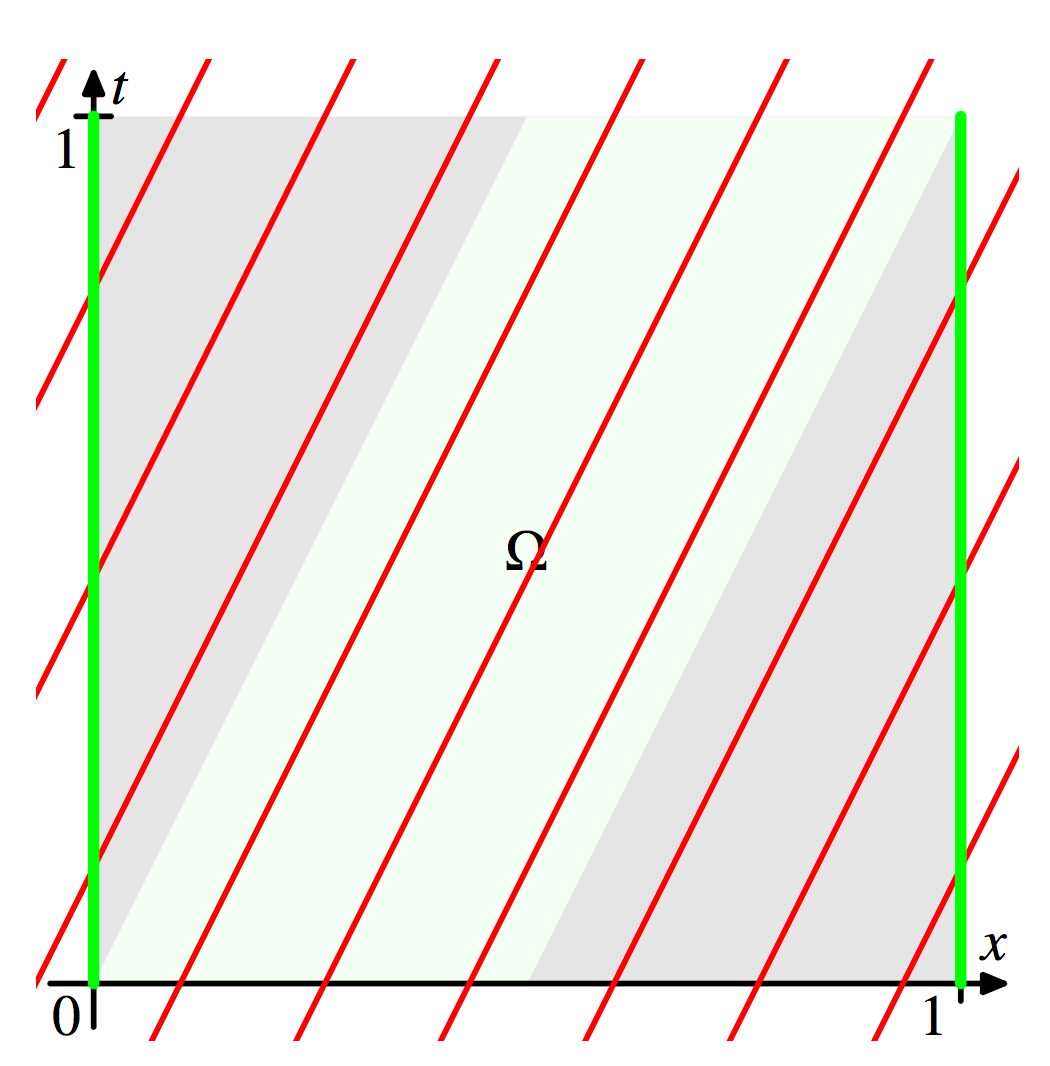
\includegraphics[width=6cm]{Content/01_theory/charakteristiken_randwerte.png}
\end{minipage}

\paragraph{Example:}~\\
\begin{enumerate}
	\item PDE with boundary conditions and domain: $\partFrac ux+2\partFrac uy=3$, \; $u(0,y)=g(y)=\sin(y) \Rightarrow u(0,y_0) = g(y_0) = \sin(y_0)$\\
	Terms in matrix form: $\begin{bmatrix}a\\b\\c\end{bmatrix}=\begin{bmatrix}1\\2\\3\end{bmatrix}$
	\item Calculate characteristics from PDE $\rightarrow$ ODE: 	$\frac {d}{dt}\begin{bmatrix}x(t)\\y(t)\\u(t)\end{bmatrix}=\begin{bmatrix}1\\2\\3\end{bmatrix}$
	\item Solve ODEs (for standard ODEs, see \ref{sec:dgls} on page \pageref{sec:dgls}.):
	$\begin{bmatrix}x\\y\\u\end{bmatrix}=\begin{bmatrix}1t+x_0\\2t+y_0\\3t+u_0\end{bmatrix}$
	\item Substitute initial conditions: $\begin{bmatrix}x\\y\\u\end{bmatrix}=\begin{bmatrix}1t+x_0\\2t+y_0\\3t+u_0\end{bmatrix}\Bigg|_{t=0}=
	\begin{bmatrix}x_0\\y_0\\u_0\end{bmatrix}=\begin{bmatrix}0\\y_0\\\sin(y_0)\end{bmatrix}$\\
	Solution of ODE is: $\begin{bmatrix}x\\y\\u\end{bmatrix}=\begin{bmatrix}1\\2\\3\end{bmatrix}\cdot t+ \begin{bmatrix}0\\y_0\\\sin(y_0)\end{bmatrix}$\\

	\item Eliminate all variables except $u,x,y$: $u=3x+\sin(y-2x)$
	\item Verification:
	Derive the result ($u=3x+\sin(y-2x)$) and substitute it into the original PDE $\partFrac ux+2\partFrac uy=3$ to check if it is satisfied.

\end{enumerate}
